%%Maximum length = smallestOf( 12,000 words, 35 pages )
%%Report file name must be "team_X.pdf" (where X is the team name)

%Your initial report set out your aims for the project which you may wish to modify in light of feedback received. The final report should detail out what you set to achieve, what you did achieve, how you achieved it, and your evaluation of your work. You are free to structure your report as you see fit, and different projects may naturally lead to different structures. An example structure for your report follows. Bear in mind that the main aim of your report is to show the examiners that you have done quality work: focus on the noteworthy, not the mundane; explain what the examiners cannot know rather than the obvious; and show that you understand your project’s weaknesses as well as its strengths.


% Apply paragraph spacing only for the main report body %
\setlength{\parskip}{1em}

\section{Introduction}
%Describe the context for the work and the problem you are addressing. Briefly summarise what you achieved in the project.

The goal of the project was to create an urban traffic simulation over the connected road network resembling ones found in real world. Such simulation would allow inspection of different traffic properties such as vehicle throughput in strategic points and possible effects of altering rules or road network topology. In addition to providing basic inspection functionality, the system would be easily extendable with extra, more complex observable properties such as pollution factors.

The project's original approach followed the cellular automata model, with the map represented as grid consisting of cells maybe occupied by a car. Shortly after initial prototype implementation the requirement for real map data was raised. The cellular automata model was found to be lacking flexibility due to fixed cell size. Such model did not pair well with the multitude of forms and combinations found in real maps, so it had to be abandoned in favour of, or rather morphed into, a more physical metric model. In this physical model vehicles bear real-life properties such as speed, acceleration, angle and position on the lane, and move according to laws of physics. The latter uncovers a potential for further model refinement. Certain key map features have inspection properties attached to them, namely vehicle counters, enabling live inspection. Data import from Open Street Map format was added, which allows for interoperability with a vast tooling and data ecosystem already available, as well as the convenience in creating synthetic test examples.

Vehicle behaviour, namely driving and reasoning about the routes, received less attention than originally anticipated. At the same time some interesting driving behaviour, such as acceleration, braking, turning and lane changing, was implemented. Though, vehicles can not be classified as agents, since interface between environment and vehicle is not that well defined, and really cars are only capable of basic reactive behaviour.

A sophisticated user interface has been created, partly to facilitate the need for visual inspection of various data available on the map, but also useful for display of the actual simulation runs (see Figure~\ref{fig:screenshot}).

\begin{figure}[H]
    \vspace{1.5em}
    \caption{Screen capture of the main application window depicting car moving at Aldwych}
    \label{fig:screenshot}
    \centering
    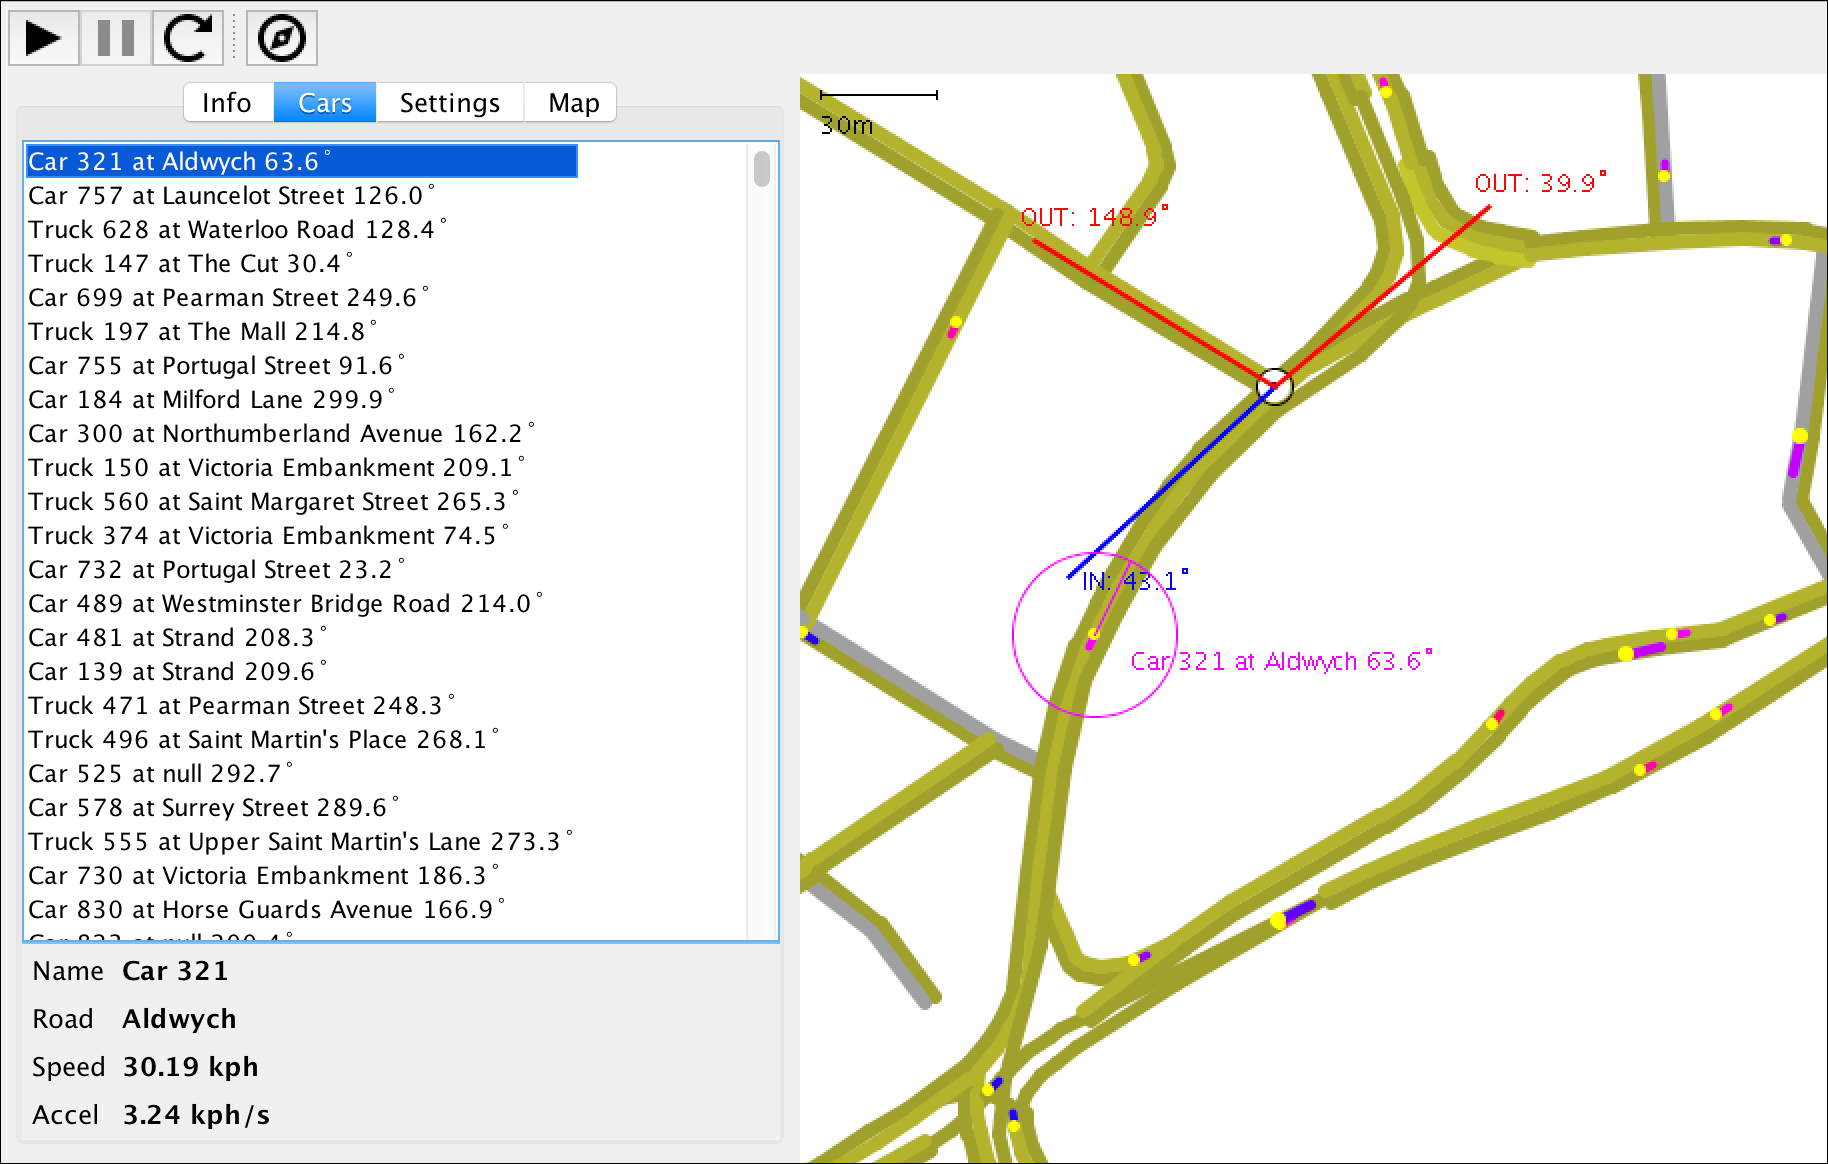
\includegraphics[width=0.75\textwidth]{figs/mainWindowWithStrand.png}
    \vspace{1.5em}
\end{figure}

\section{Review}
%Describe related work.

A wide array of traffic modelling systems have been developed, either using classical software modelling (micro and macro), or with innovative and hybrid approaches (MESO and agent-based) \cite{Hawick2009}. Both categories have their own advantages and disadvantages. In this chapter their strengths and weaknesses will be summarised.

\subsection{SUMO}

Simulation of Urban Mobility (SUMO) is a popular open-source road traffic simulation software which was implemented using the aspects of microscopic flow behaviour model. The main idea is to simulate complex road networks. Any road network can be modelled in the system through import from various sources\cite{Ismail2012}. SUMO supports simulation of ways, junctions, traffic lights, routes. Options available in SUMO include physical and logical properties of vehicles and traffic distribution based on them. SUMO is an open and well studied software in addition to being implemented in different national projects such as DRIVE C2X, COLOMBO and AMITRAN\cite{TransportResearchattheGermanAerospaceCentre2016}.

Although used widely, SUMO is a complex piece of software with a steep learning curve\cite{Ismail2012}.

\subsection{AIMSUN}

AIMSUN is another popular and well studied commercial traffic simulation software created by Transport Simulation Systems (Spain). It is commonly classified as a micro-model simulator. Nevertheless, it also supports macro and meso models. A user has an ability to configure specific mode and manage the parameters of the traffic flow\cite{Hawick2009}. Supporting a dynamic simulation AIMSUN can operate with larger road networks as highways, freeways, and ring roads. By default it has simulation scenarios which allow users to run experiments with specific parameters.

Another feature supported by AIMSUN is 3D simulation which provides detailed point of observation from any angle.

One of the significant disadvantages of AIMSUN is that users are required to write scripts specifying the flow and the the network model. Also, as it was found, the usage of 3D mode dramatically affects the performance \cite{Hawick2009}.

\subsection{SATURN}

SATURN (Simulation and Assignment of Traffic to Urban Road Networks) is a macroscopic-based traffic simulator created by the Institute for Transport Studies in the University of Leeds. It is popular in Europe and the UK. SATURN aims to simulate public transport traffic in urban areas. Since SATURN employs a macro-model, it allows observation of the large scale impact public transport can have. Possible parameters can be cost and duration of journey, vehicle price and configuration of fare zones. PT-SATURN, an addon, is available which provides simulation of the passenger behaviour within public transport. Problems like which transport to choose, where to travel, what route to take can also be incorporated in the simulation\cite{Shires2006}.

\subsection{Summary}

Research highlighted different issues that exist within the models. The advantage of each model dramatically depends on their intended purpose, therefore these must be selected based on the required granularity.

\section{Requirements and Design}
%Describe the requirements you set for your project at the beginning and the design you have taken for your project. Focus on why you decided to tackle the problem in the way you did, and what effects that had on the design. You may also wish to mention the impact of team-working on your requirements and design.

There were no formal requirements specified at any stage. Instead, the team followed the agile requirements process with no dedicated product manager. In essence, requirements were created by piling possible improvements and things of possible interest into the backlog task section, which were evaluated and taken for implementation based on their priority. At the same time, there were basic minimal requirements of creating a working product with a GUI displaying vehicles moving in map setting.

The requirements drove the evolution of the model and vice versa. The original cellular automata model was rather limiting, so with the introduction of enhanced model more things became possible (i.e. cars display in an angle following the road angle).

Naturally, implementation of some features took place earlier, defining ongoing possibilities for other features to be implemented. As such, free-form junctions demanded some test fixtures, which in turn led to requirement for loading external data files. At the same time, the GUI started to serve as a sort of visual inspector and debugger leading to an ever evolving design.

With such an evolutionary approach to requirements the specific attention has been paid to internal structure and architecture enabling easier new features implementation. Design methodologies such as separation of concerns, modularization and design patterns were used to make software more robust and maintainable in the course of unforeseen changes.

Actual implemented features are listed in Table \ref{table:functionalities} in Section \ref{sec:projectEvaluation}.

\section{Implementation}
%Describe the most significant implementation details, focusing on those where unusual or detailed solutions were required. Quote code fragments where necessary, but remember that the full source code will be included as an appendix. Explain how you tested your software (e.g. unit testing) and the extent to which you tested it. If relevant to your project, explain performance issues and how you tackled them.

Whilst test driven development process was selected by the team initially, usage of proper unit testing declined over time due to looming deadlines. Still, regular practice of writing tests for some parts of the system, especially core and complex ones, persisted.

%%%%%%%%%%%%%%%%%%%%%%%%%%
% Alex part
%%%%%%%%%%%%%%%%%%%%%%%%%%
%%%%%%%%%%%%%%%%%%%%%%%%%%
\subsection{Technology and Libraries}

Java Standard Edition version 1.8 was chosen as an implementation platform, since Java is a language familiar to all team members. At the same time it provides a Graphical User Interface framework and an excellent tooling support. Gradle\footnote{Gradle is a modern build system for Java in tight integration with Groovy http://gradle.org} was used as a build system to automate builds on Travis continuous integration server and also to produce various artefacts.

There were no external libraries used for the actual application code, except for the Java standard runtime library (rt.jar).

In order to enable more convenient unit-testing, following libraries were used:
\begin{enumerate}
    \item Junit 4 as an actual test runner
    \item Mockito\footnote{https://code.google.com/archive/p/mockito/} - easy mocks in java. Enables better separation of concerns and fluent invocation verification patterns
    \item Fest assertions\footnote{https://github.com/alexruiz/fest-assert-2.x/wiki/One-minute-starting-guide} - library enabling writing comprehensive and convenient assertions
\end{enumerate}

In order to work with OpenStreetMap files, appropriate standard OSM tools were used (namely, JOSM and osmosis), as detailed further in the report.

%%%%%%%%%%%%%%%%%%%%%%%%%%
% Alex part
%%%%%%%%%%%%%%%%%%%%%%%%%%
%%%%%%%%%%%%%%%%%%%%%%%%%%
\subsection{Map Data Import}
According to the requirements, the software would need to be able to model traffic behaviour in real-like road networks. In addition to the organic requirements, there were synthetic ones, demanded by various test fixtures for all application components from actual vehicle behaviour to individual lane visualisation.

Decision was made to use already-available public-domain ordnance data from OpenStreetMap\footnote{OSM data is available under ODbL license, see http://www.openstreetmap.org/copyright} (OSM)  worldwide project. It was a natural decision since data is available for all the world, and is collaboratively created by a multitude of users. OSM has a strong technical community and ample documentation. Finally, it contains all the most important data which may be required for traffic simulation. Data files are available in well-known XML format\footnote{Having said that, there is no official XML type specification due to main software pieces in ecosystem vaguely interpreting different cases: http://wiki.openstreetmap.org/wiki/OSM\_XML}. As an extremely useful side-effect, using such widely available data allows a user to obtain a map of the area of particular interest for simulation following simple steps, so it greatly adds to the practical value. At the same time, the implementation of such loading turned out to not be straightforward due to data originating from many human contributors bearing all the inconsistencies and errors possible for vaguely defined data.

OSM format defines three main types of objects: nodes (points having coordinates), ways (polylines, sequences of nodes) and relations (types of relationships between other objects). These are extensively tagged to represent all the complex settings of the real-world mapping. For example: a way (sequence of node references) with tag type equal to primary and lanes equal to 4 would mean a two-way primary road. However a way with type building represents a building on the map, and should be a closed polygon. All the objects have their ID attached to them via tags.

Following is a compact overview of the pipeline the data follows from the OpenStreetMap file downloadable from the internet to the actual simulation process:
\begin{itemize}
    \item Stage 1. Using standard OSM software tools (Osmosis, JOSM), prepare the excerpt from large data set, which is suitable for simulation.
    \item Stage 2. Using obtained OSM XML file, load a set of Descriptor objects:
    \begin{itemize}
        \item Collection of road descriptors: objects describing roads, with number of lanes in each direction
        \item Collection of junction descriptors: object describing junctions, and their connection with roads
        \item Generic knowledge about map setting, such as map geographical bounding box.
    \end{itemize}

    \item Stage 3. Using descriptor objects, construct in-memory graph representation of the road networks:
    \begin{itemize}
        \item Create roads from descriptions. Create individual lanes within the roads. Offset lanes accordingly.
        \item Create junctions from descriptors.
        \item Link roads and junctions using junction descriptors. Link on individual lanes. Compute possible inflow and outflow paths for junctions to save time in simulation run.
        \item Walk the graph and attach traffic generators and receivers to the edges not yet connected.
    \end{itemize}

    \item Stage 4. Run the traffic simulation on the created map.
\end{itemize}

%%%%%%%%%%%%%%%%%%%%%%%%%%
% Alex part
%%%%%%%%%%%%%%%%%%%%%%%%%%
%%%%%%%%%%%%%%%%%%%%%%%%%%
\subsubsection{Preparing Data File}
First of all, a user needs to decide on the actual geographical area they want to perform the simulation of. The area is uniquely defined by 2 pairs of geographical coordinates: (south-west lat, long) - (north-east lat, long). After that, user needs to either download the full planet.osm file (containing whole OSM data set), or an area excerpt containing the area of interest\footnote{Geofabrik is a reliable source for OSM excerpts with fresh data http://www.geofabrik.de}.

Following is the osmosis tool command line, which combines both cut and filter steps into single run:
\begin{lstlisting}
$ osmosis --read-xml file=INPUT_LARGE_FILE.osm enableDateParsing=no
        --tf accept-ways highway=trunk,motorway,primary,secondary,tertiary
            ,motorway_link,trunk_link,primary_link,secondary_link,tertiary_link
        --bounding-box bottom=48.867844 left=2.289727 top=48.879678 right=2.304442 completeWays=yes
        --used-node
        --write-xml OUTPUT_FILE.osm
\end{lstlisting}
'completeWays=yes' key is of specific interest. When osmosis attempts bounding box reduction, and finds a way which is located both inside and outside the bounding box, its default behaviour is to terminate the way at the last node within the box. When applied to real life data, this yielded ugly results, sometimes terminating road network segment where it should not terminate. As a counter action, this key is used to include all the ways which are within, or intersect with, the bounding box rectangle.  As a result, the OSM XML file with some ways spanning outside of the box is obtained which may be opened directly from within the user interface of the Traffic Simulator system, or edited in any standard OSM file editor such as JOSM.

Figure \ref{fig:thirdPartyToolsOSMPreparation} summarizes steps performed during preliminary file preparation process.
\begin{figure}[h]
    \vspace{1.5em}
    \caption{OpenStreetMap file preparation}
    \label{fig:thirdPartyToolsOSMPreparation}
    \centering
    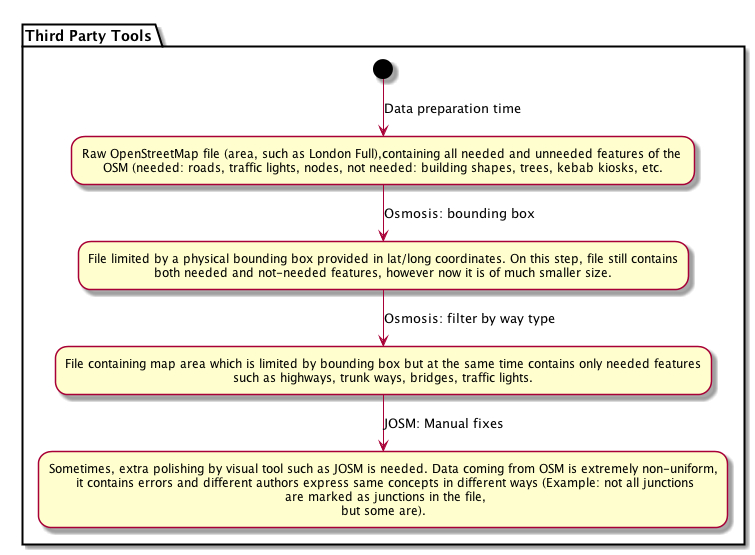
\includegraphics[width=0.8\textwidth]{../../uml_diagrams/thirdPartyToolsDataLoading.png}
    \vspace{1.5em}
\end{figure}


%%%%%%%%%%%%%%%%%%%%%%%%%%
% Alex part
%%%%%%%%%%%%%%%%%%%%%%%%%%
%%%%%%%%%%%%%%%%%%%%%%%%%%
\subsubsection{Descriptors Creation from the OSM File}
After the actual simulation map OSM file is created, it may be opened directly from the traffic simulator. In order for the data contained in an XML file to be used, it first needs to be read, parsed and adopted into the internal format on top of being linked into the in-memory graph.

Actual parsing of the XML file has been implemented using standard java SAX\footnote{Simple API for XML, https://docs.oracle.com/javase/7/docs/api/javax/xml/parsers/SAXParser.html} parser. When choosing between the DOM and SAX parsing, the latter was selected as the DOM has significantly larger memory requirement\footnote{DOM establishes the whole document as a tree in memory and exposes many complex APIs and methods for manipulating that tree which are not needed for the loading data case}. SAX employs event-driven XML parsing model: when the parser encounters a new element, closing element, an attribute or text blocks, it invokes appropriate methods on handler object. In order to listen to these events, class OsmSaxHandler has been created.

First, the bounding box representing the actual geographical rectangle containing all the places of interest is read. Whilst OSM operates in geo-coordinates, the actual simulation happens on a flat positive Cartesian coordinate system. All objects have coordinates as offset from zero point by the x and y axis. Figure \ref{fig:coordinateConversions} provides an overview of what coordinate systems are used across the traffic simulation system. At this stage of parsing, the conversion operator is initialized by the offset to translate geographical coordinates to meters offset.

\begin{figure}[h]
    \vspace{1.5em}
    \caption{Coordinate systems used in the traffic simulation system}
    \label{fig:coordinateConversions}
    \centering
    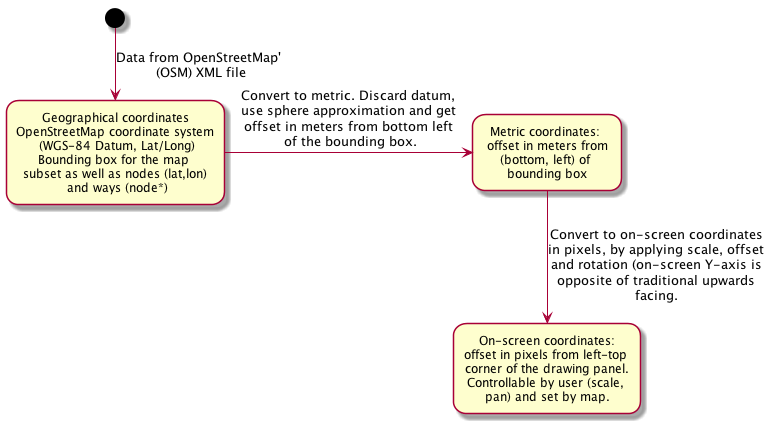
\includegraphics[width=0.8\textwidth]{../../uml_diagrams/coordinateSystems.png}
    \vspace{1.5em}
\end{figure}

 Since OSM has a small set of basic objects to express mapping data, roads are expressed as <way> elements, containing a sequence of references to nodes which, effectively, forms a polyline. There is no notion of road width as such in the original data. Only the number of lanes and whether the road is one way or not is recorded in it. The design decision has been made to have the default lane width set to the standard 3.2 meters\cite{Council2016}. Using lane width, one-way flags and number of lanes in road, the physical representation of the road is created.

\begin{figure}[h]
    \vspace{1.5em}
    \caption{Polyline creation and visualisation stages}
    \label{fig:roadAndLanesPolylines}
    \centering
    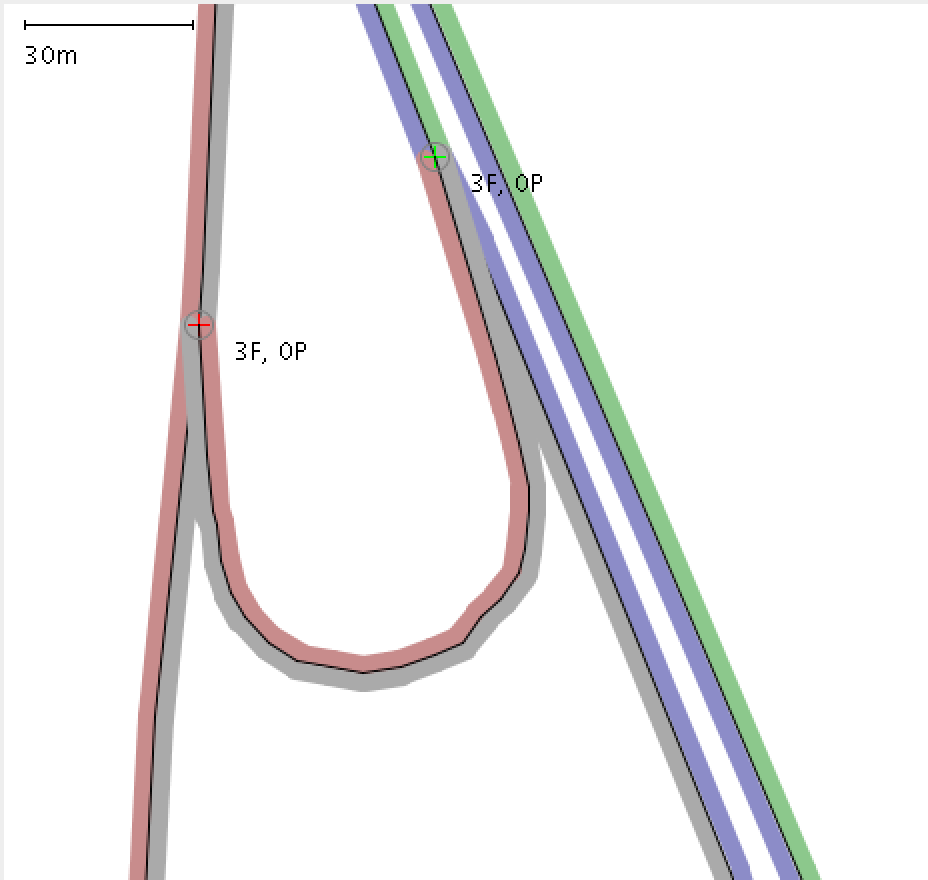
\includegraphics[width=0.4\textwidth]{figs/road/road_polyline.png}
    \hspace{0.2em}
    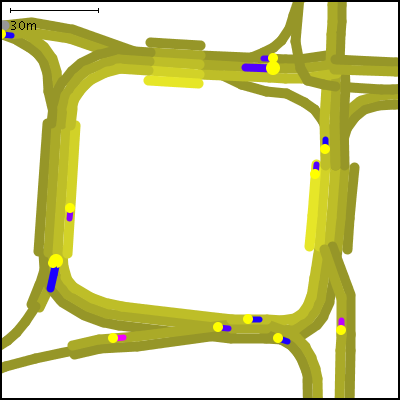
\includegraphics[width=0.4\textwidth]{figs/road/road_lanes.png}
    \vspace{1.5em}
\end{figure}

At the same time, XML data file provides enough information to construct a road central axis polyline. After this polyline is available, the individual lanes' own polylines are constructed using positive or negative shifts along the normal vector to the current segment. This depends on the position of the lane in the road. Figure \ref{fig:roadAndLanesPolylines} shows an overview of the process: on the left the road's central axis polyline is visible (thin black hairline), on the right the more complex junction with multiple lanes, constructed using the method mentioned before is visible.

For the simulation to run smoothly, the road network needs to be represented as a well-formed graph data structure. In order to facilitate the requirement, post-processing is applied to the road and junction descriptions collected from the XML file. Roads containing junction node as a non-edge polyline node were split - one part terminating at junctions whilst the other starting from them. This allowed for future uniformity of the movement logic. The vehicle simply follows high-level graph while making low-level decision on acceleration and deceleration and is naturally transported to the next feature (graph node) as long as it finished its travel on the previous one.

Unfortunately, the collaborative nature of OpenStreetMap data leads to multiple ambiguities:
\begin{itemize}
    \item Human factor. Same real-world concepts, such as junctions, road connections and pedestrian crossing, happen to be expressed in a different way in XML files by different contributors. For example, the node has a tag which indicates that it is a junction, however not all real crossings do have this label attached to the crossing node. The design decision has been made to default to the least common denominator. For example: a situation when a node is identified by the same id and is contained in two 'ways' is a crossing.
    \item Eventual data consistency. In some cases the OpenStreetMap data contains simple errors or misconceptions which lead to a concrete change in coding practice. For example: instead of throwing an exception when meeting an inconsistent data situation, the load layer attempts to fix it to its best ability whilst keeping detailed logs of the causes and related data excerpts for human inspection. If the node referenced in the road polyline is not found in data file, the data loading is not terminated - some nodes just happen to be cut off by processing, and some are erroneously referenced. It seems that official OSM software is tolerant to these inconsistencies as well and presence of such ill-formed data is one of the causes of the absence of the formal data specification.
\end{itemize}

The approach of importing OpenStreetMap data was eventually found to have some similarities to the one employed in SUMO, with some guess work as well as a high tolerance to data file errors. At the same time, SUMO employs much more complex and rich data standard for its simulation setting.

The following problems were encountered and solved during the implementation of the XML data loading:
\begin{itemize}
    \item Coordinate conversions: since the Mercator projection\footnote{https://en.wikipedia.org/wiki/Mercator\_projection} with spherical geoid simplification is used, there is a certain degree of inaccuracy in the coordinates converted to meters offset.
    \item Splitting roads when they happen to cross a junction in the middle (see Figure~\ref{fig:roadSplitting}): as it's a rather technically complex, it leads to a cumbersome algorithm. The reason being that the processing of the roads and junctions happened at the same time so, in case a split is required, the references must be found and updated to match the newly created parts based on the original road.
    \item Link descriptors: initially, it was anticipated that another type of descriptor - <LinkDescription> - would be created to mark the places where two parts of the road are connected (for example, pedestrian crossing on a straight road). However, after the implementation of the data loading found a need for road splitting, Link descriptors were abandoned in favour of the more general idea of junction descriptors that had only two roads connected. Otherwise, the edge-case situation of a link descriptor created in a geographical point, which was later to be found to be in the middle of another road, led to an overly complex code. This conversion positively reflected on the overall design of the system and followed the "keep it simple" rule. At later stages, the graph construction and actual simulation were found to be working perfectly with "junctions with two roads" instead of a link.
    \item Lane construction: deriving from a single zero-width road polyline a set of lane polylines which are offset into appropriate direction (perpendicular to the segment).
\end{itemize}

\begin{figure}[h]
    \vspace{1.5em}
	\caption{Example of road being split at junction}
	\label{fig:roadSplitting}
	\centering
	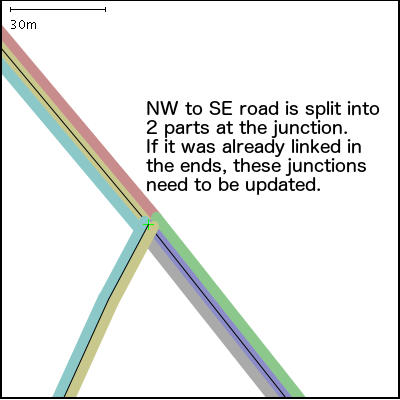
\includegraphics[width=0.4\textwidth]{figs/junction/road_splitting.png}
    \vspace{1.5em}
\end{figure}


At the same time, extending the map data loader with extra functionality, such as maintaining pedestrian crossing information or traffic lights information, would provide system with some benefits, there is a clear potential for improvement on this side.

\subsection{Graph Construction}

Graph construction is done prior to the simulation running rather than during (Just In Time). This approach moves the performance penalty away from the live simulation leaving some overhead for a large workload with heavy maps. It also, conceptually, makes for easier storage of map states on every tick as, once the graph is set, the only changes are in the counters, link states (e.g.: such as traffic lights being red/green) and the map objects travelling on the graph.
From the previously created descriptors, the graph constructor creates the features and links of the graph and actually connects them toghether in memory in this order (see Figure~\ref{fig:graphConstructSeqDiag} and ~\ref{fig:roadConstructSeqDiag} in Appendix~\ref{sec:roadConstructionSequences}):
\begin{enumerate}
	\item Roads, their directed lane groups and individual lanes are created,
	\item Junctions are created and the roads branching off them connected,
	\item Traffic generators are placed.
\end{enumerate}

\subsubsection{Feature Creation and Linkage}

Originally the graph was kept abstract with features connected via links (see Figure~\ref{fig:FeatureConnect}). These features could be either junctions or roads. Roads were connected as whole features (see Figure~\ref{fig:RoadsOriginal}).

\begin{figure}[h]
	\vspace{1.5em}
    \caption{Original design with Features and Links}
    \label{fig:FeatureConnect}
    \centering
    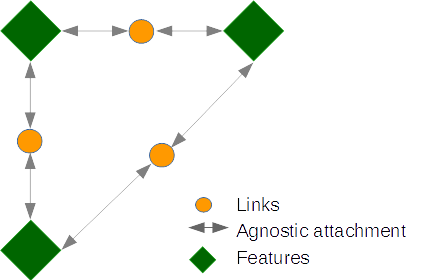
\includegraphics[width=0.50\textwidth]{figs/graphConstruction/OriginalConnections.png}
    \vspace{1.5em}
\end{figure}

\begin{figure}[h]
    \vspace{1.5em}
    \caption{Roads in the original high abstraction design}
    \label{fig:RoadsOriginal}
    \centering
    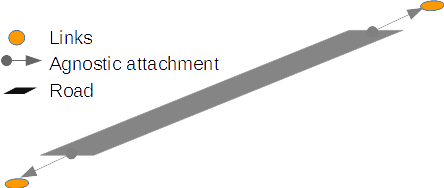
\includegraphics[width=0.45\textwidth]{figs/graphConstruction/OriginalRoads.png}
    \vspace{1.5em}
\end{figure}

As more work was done it became clear that this high level of abstraction on the graph was not going to be practical. Thus it progressed into having roads broken into groups of directed lanes. This allows the lanes to be connected individually in a directed fashion in the graph. Roads are now composed of lane groups that are, themselves, composed of single lanes (see Figure~\ref{fig:RoadsFinal}).

\begin{figure}[h]
	\vspace{1.5em}
  	\caption{Roads, Directed lane group and lanes}
  	\label{fig:RoadsFinal}
  	\centering
	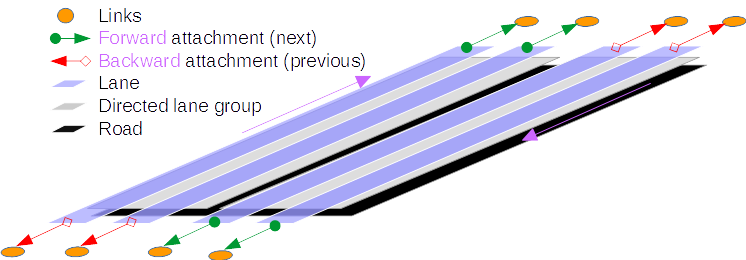
\includegraphics[width=0.75\textwidth]{figs/graphConstruction/Roads.png}
  	\vspace{1.5em}
\end{figure}	

Although roads and lane groups are not directly connected up in the graph, the belonging lanes can back reference those enabling travelling objects to access their properties. I.e.: A vehicle on a lane can find out the Road's name or ID as well as what direction it belongs to.

Junctions were developed around this exploded view of the road feature. Lanes are connected up to junctions via special junction-specific links that give access to available paths from that particular entry point with the <getLinks()> method for any passing objects (see Figure~\ref{fig:junction}).

\begin{lstlisting}[language=Java]
    public List<Link> getLinks() {
        try {
            return junction.getNextLinks(super.getID());
        } catch (JunctionPathException e) {
            LOG.log_Fatal("No exit link from the junction were found! i.e.: Car is stuck!");
            return Collections.emptyList();
        }
    }
\end{lstlisting}

Paths are calculated after lane linkage has been done. All entry points are connected up to all exit points unless it double backs on the same road (u-turn) (see Figure~\ref{fig:junction}). The paths are stored in a <TrafficBehaviour> object as lists for each entry point ID inside a map:

\begin{lstlisting}[language=Java]
	private Map<ID, List<ID>> outflowPaths;
\end{lstlisting}

\begin{figure}[!h]
	\vspace{1.5em}
  	\caption{Junction}
  	\label{fig:junction}
  	\centering
	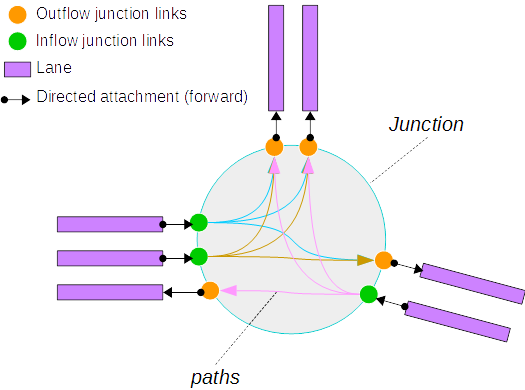
\includegraphics[width=0.6\textwidth]{figs/graphConstruction/Junction.png}
  	\vspace{1.5em}
\end{figure}

\subsubsection{Traffic Generators}

Traffic generators were originally designed to only produce traffic but evolved to also take receipt of it thus taking on the responsibility of deleting vehicles as they exited the boundaries of the simulated map. This ensures that vehicles disappear at the designated boundaries and cannot keep going forward (graphically). This also allows to keep track on the numbers of vehicles produced and received at those points (see Figure~\ref{fig:boundaryTF}).

During development two corner cases were encountered:
\begin{enumerate}
	\item Junctions where there were only incoming lanes connected to,
	\item Junctions where there were only incoming lanes connected to save for one road.
\end{enumerate}

In the first case, vehicles from all lanes had no where to go. In the second case, where the traffic came into the junction from the lone road with both direction included, the traffic had also no where to go since the only way out would have been a u-turn which is not allowed.
Both were dealt by placing traffic generators on those special case junctions to take in the orphaned traffic (see Figure~\ref{fig:junctionTF}).

\begin{figure}[!h]
	\vspace{1.5em}
	\centering
	\begin{minipage}[t]{0.60\textwidth}
  		\caption{Traffic Generators at Map boundaries}
  		\label{fig:boundaryTF}
  		\centering
		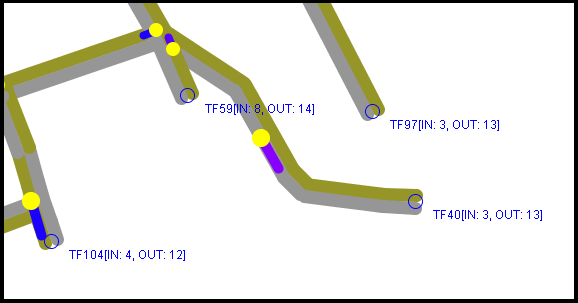
\includegraphics[width=1\textwidth]{figs/trafficGenerator/generate-receive.png}
	\end{minipage}\hfill
	\begin{minipage}[t]{0.35\textwidth}
  		\caption{Junction Traffic Generator}
  		\label{fig:junctionTF}
  		\centering
		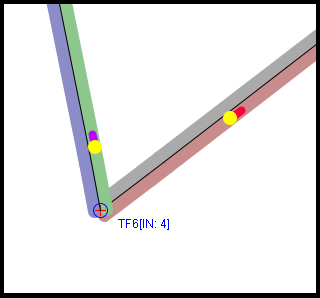
\includegraphics[width=1\textwidth]{figs/trafficGenerator/inflowOnly.png}
	\end{minipage}
	\vspace{1.5em}
\end{figure}

By having traffic generators automatically placed at any dangling links, any OSM data issues or inconsistencies can be seen in the graphical representation of the map at a glance. It also acts as a safety net when these occur by ensuring that all ends are connected to something and traffic is kept within the boundaries of the map (i.e.: no escaping vehicles). Another positive side effect is that, during construction of the graph, any island features (be it orphaned features that are unconnected or actual geographic islands) are ensured to have traffic running on them. For example see Figure~\ref{fig:islandReal}.

\begin{figure}[!h]
	\vspace{1.5em}
  	\caption{Island problem resolution}
  	\label{fig:islandReal}
  	\centering
	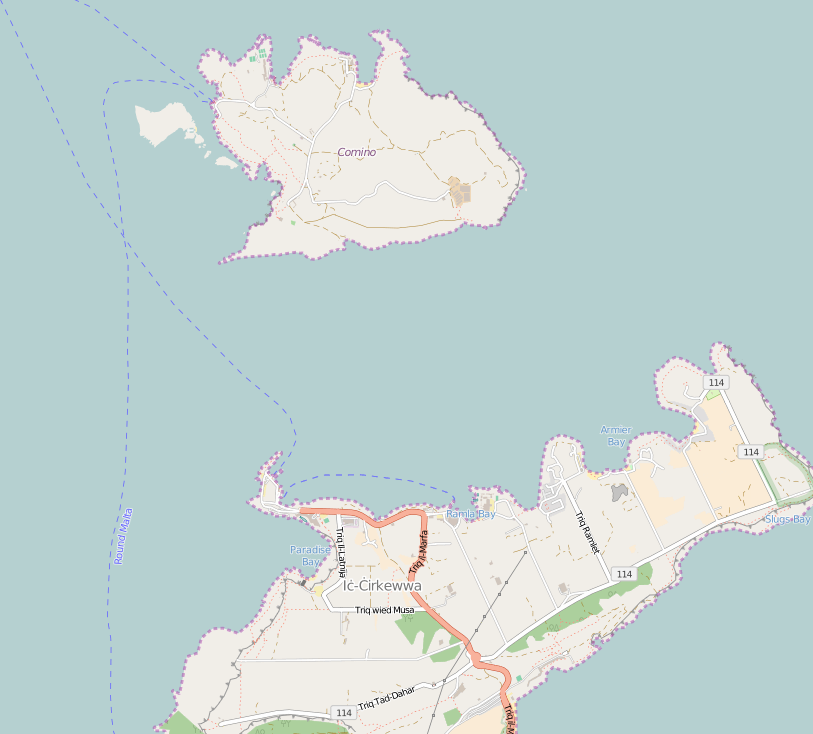
\includegraphics[width=0.4\textwidth]{figs/trafficGenerator/IslandExample_realmap.png}
	\hspace{0.2em}
	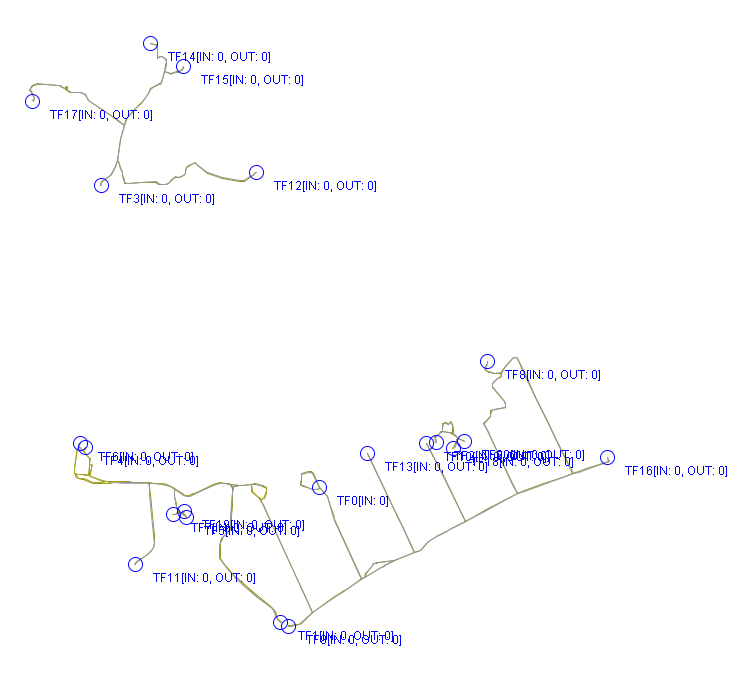
\includegraphics[width=0.40\textwidth]{figs/trafficGenerator/IslandExample_simmap.png}
  	\vspace{1.5em}
\end{figure}

\subsubsection{Caveats}
There is one problem stemming from the way the OSM data is laid out. It manifests itself most commonly in round-about situations. In cases, some incoming lanes belonging to a road going into a round-about cannot be connected in a directed fashion as the entry into the roundabout goes contra-way to that road. A good example of this issue is the Waterloo roundabout (see Figure~\ref{fig:roundAbout}).

\begin{figure}[!h]
	\vspace{1.5em}
  	\caption{Round-about problem}
  	\label{fig:roundAbout}
  	\centering
	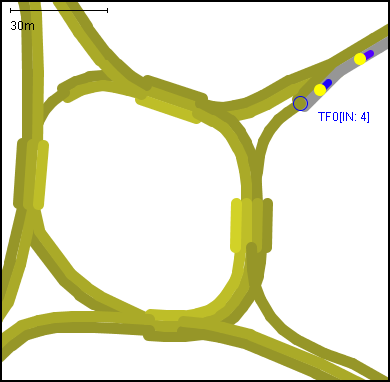
\includegraphics[width=0.4\textwidth]{figs/graphConstruction/RoundAbout1.png}
	\hspace{0.2em}
	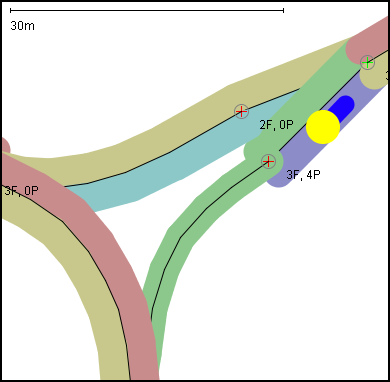
\includegraphics[width=0.40\textwidth]{figs/graphConstruction/RoundAbout2.png}
  	\vspace{1.5em}
\end{figure}

The most obvious way to deal with this would be to detect roundabouts at the post OSM data import and recreate a viable set of descriptors that would not produce this errors. This would, however, add an additional overhead as all link and feature descriptors would need to be examined alongside their geographical relationships. At the moment, since only incoming lanes are detected at the point of connection, a traffic generator is automatically added to the junction to take receipt of the traffic.

%%%%%%%%%%%%%%%%%%%%%%%%%%
% Alex part
%%%%%%%%%%%%%%%%%%%%%%%%%%
%%%%%%%%%%%%%%%%%%%%%%%%%%
\subsection{Map visualisation}
As soon as map is constructed, a representation of the road network graph which acts as a base for simulation is placed in memory. Roads, consisting of lanes, connect up to junctions, roads and lanes have polylines. All the coordinates in simulation space are provided in meters offset Cartesian coordinates - that is, horizontal and vertical meters offset from (0,0) bottom left point, as outlined in Figure \ref{fig:coordinateConversions}.

In order for these objects to be visualized, their coordinates in simulation space need to be transformed to the on-screen coordinates. Java graphics API uses pixel coordinates, with origin point being top-left, and vertical axis pointing down.

In addition to that, user is provided with comprehensive tools to control the view-port: zoom in and out with mouse scroll and pan with mouse drag gestures. These gestures control offset point and scale factor of the meters to screen coordinate conversion function. In addition to being natural, such coordinate system separation (meters offset in simulation and pixels in view), allow to inspect the details of the simulation even when it is paused, while also providing an ability to see overall picture.

Whilst being useful to a user, such conversion poses not only technical, but also design challenges. Since the primary interest is on vehicles and UI supports different scale, there was a need to come up with design decision to allow car inspection on different zoom levels. When the zoom level allows for rather detailed drawing of vehicles, they are representing in their bounding rectangles. When user zooms out too far, cars collapse to dots to make the overall road network visually readable. Figure \ref{fig:mapZoomOptions} has both options on display.
\begin{figure}[!h]
    \vspace{1.5em}
    \caption{Map zoom options}
    \label{fig:mapZoomOptions}
    \centering
    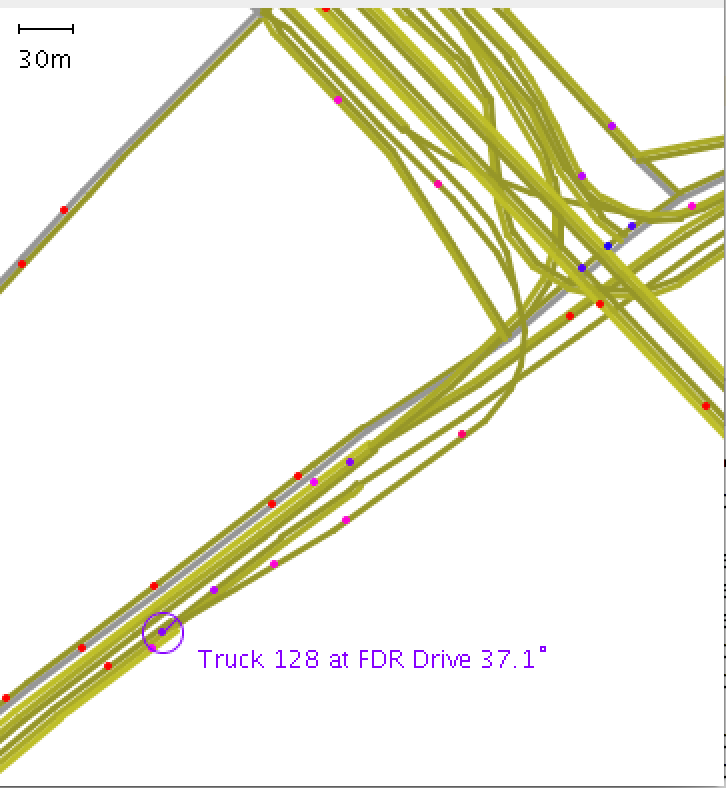
\includegraphics[width=0.4\textwidth]{figs/road/zoom_dots.png}
    \hspace{0.2em}
    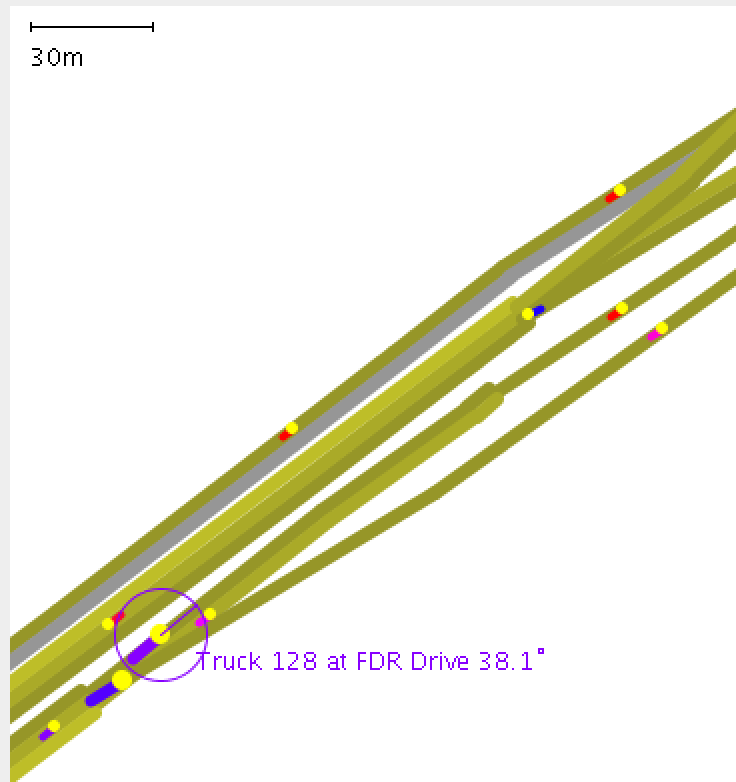
\includegraphics[width=0.4\textwidth]{figs/road/zoom_cars.png}
    \vspace{1.5em}
\end{figure}


In addition to display functionality, the map provides interactive feedback. When the vehicles are visible, clicking it would select the vehicle both in inspection pane and on-map. When junctions are visible, clicking on a particular junction would reveal its incoming and outgoing road angles. While helpful for an inspection of map particularities, this feature was extremely useful for debugging vehicle movement code. Such interlinked functionality between multiple representations (vehicle list and the map panel, map feature list and map panel and vice versa) is possible due to implementation of Model-View-Controller design pattern in the UI section. Figure \ref{fig:guiMVC} displays class diagram for GUI module of the traffic simulation system.

\begin{figure}[h]
    \vspace{1.5em}
    \caption{Graphical user interface class diagram: MVC pattern.}
    \label{fig:guiMVC}
    \centering
    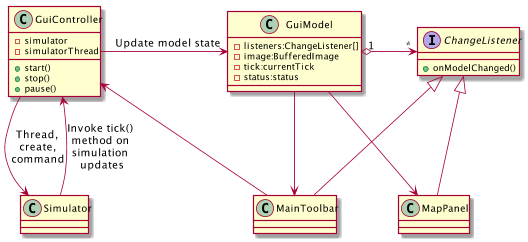
\includegraphics[width=0.75\textwidth]{../../uml_diagrams/GUI.png}
    \vspace{1.5em}
\end{figure}

\subsubsection{Optimizations}
For the simulation to run smoothly from the visual standpoint, it needs to update frames often. The overall user experience is affected by two bulky processes:
\begin{itemize}
    \item Simulation. Happens in meters offset coordinate space, this is the where the logic of the simulation happens - vehicles move along the lanes, make and implement decisions of changing lanes, accelerating and decelerating. Simulation happens in a separate background thread, as soon as one time-step of simulation is completed, simulator invokes GuiModel's callback method, which leads to the model change event to be sent to all subscribed listeners. The event is posted on the UI thread.
    \item Visualisation. When the change event is received in MapPanel, it does the job of drawing the actual simulation objects on screen, applying the coordinate conversion throughout. Visualisation happens on UI thread. Actual drawing is performed not on a panel, but on an in-memory image, which allows for future extraction of visualisation code to another thread as well.
\end{itemize}

Since the data set may be quite big, some optimizations were introduced to improve overall experience:
\begin{itemize}
    \item Limiting frame rate. There is no practical point drawing the image more often than user can normally understand, so the extra unneeded requests for draw are simply omitted:
    \begin{lstlisting}[language=java]
        public void redraw() {
            if (System.currentTimeMillis() - lastDrawnTimestamp < 1000 / MAX_FRAME_RATE) {
                LOG.log_Warning("Skipping drawing because of FPS limitation.");
                return;
            }
            lastDrawnTimestamp = System.currentTimeMillis();
            // ...
            // Actual drawing code.
    \end{lstlisting}

    \item Caching the static objects image (roads, lanes, junctions etc.) into another in-memory image and only re-drawing it when the viewport parameters such as zoom or scale, or visualisation parameters change. The invalidation check is performed with the custom hash function taking model and viewport model as arguments. Listing below provides a pseudo-code for lazy static objects draw optimization:
    \begin{lstlisting}[language=java]
        // ... checking if the viewport has changed somehow:
        if (lastViewportHashcode != model.getViewHashCode()) {
            // saving hashcode of the model+viewport just drawn for future check
            lastViewportHashcode = model.getViewHashCode();
            Graphics2D roadGraphics = (Graphics2D) roadsImage.getGraphics();
            //...
            drawAllRoads(roadGraphics);
            primitives.drawScaleOf30Meters(roadGraphics);
        }
        // regardless of change, stamp over the cached image of roads onto resulting image
        graphics.drawImage(roadsImage, 0, 0, null);
    \end{lstlisting}
    \item Extensive caching of smaller helper object (java.awt.Stroke, java.awt.Color). Since most of the drawing is using line widths dependent on the zoom level, it is beneficial to store static objects such as colors and stroke styles in caching maps for future re-use.
    \begin{lstlisting}[language=java]
        private Stroke getStrokeByWidthPixels(int width) {
            if (!strokeCache.containsKey(width)) {
                strokeCache.put(width, new BasicStroke(width, ...));
            }
            return strokeCache.get(width);
        }
    \end{lstlisting}


\end{itemize}


%%%%%%%%%%%%%%%%%%%%%%%%%%
% Alex part
%%%%%%%%%%%%%%%%%%%%%%%%%%
%%%%%%%%%%%%%%%%%%%%%%%%%%
\subsection{Traffic simulation}
Actual traffic simulation requires an already completed and linked simulation map: an in-memory data graph data structure consisting of different map features, such as roads, junctions or traffic generators. Simulation has certain parameters, such as duration of single simulation step (tick), total number of ticks to run and simulation time start. Notion of simulated time is maintained - in addition to discrete tick number, each moment of time contains a simulated time stamp. This may be required in future for more complex behaviour, such as changing environment perception parameters according to the time of the day, or profiling the traffic load to the real-like commute patterns.

\subsubsection{Simulation loop and time}
Simulation is performed in discrete steps. On each simulation steps a simulation timestamp (tick) object is created and passed down to all the interested listeners, which need to implement ISimulationAware interface. Each of them does what is needed on that level. For example, traffic lights might change their state basing on a tick, cars may change their speed, position and acceleration, traffic generators may insert the new cars onto connected outflow lanes.

\begin{figure}[h]
    \vspace{1.5em}
    \caption{Simulation class diagram.}
    \label{fig:simulationClassDiagram}
    \centering
    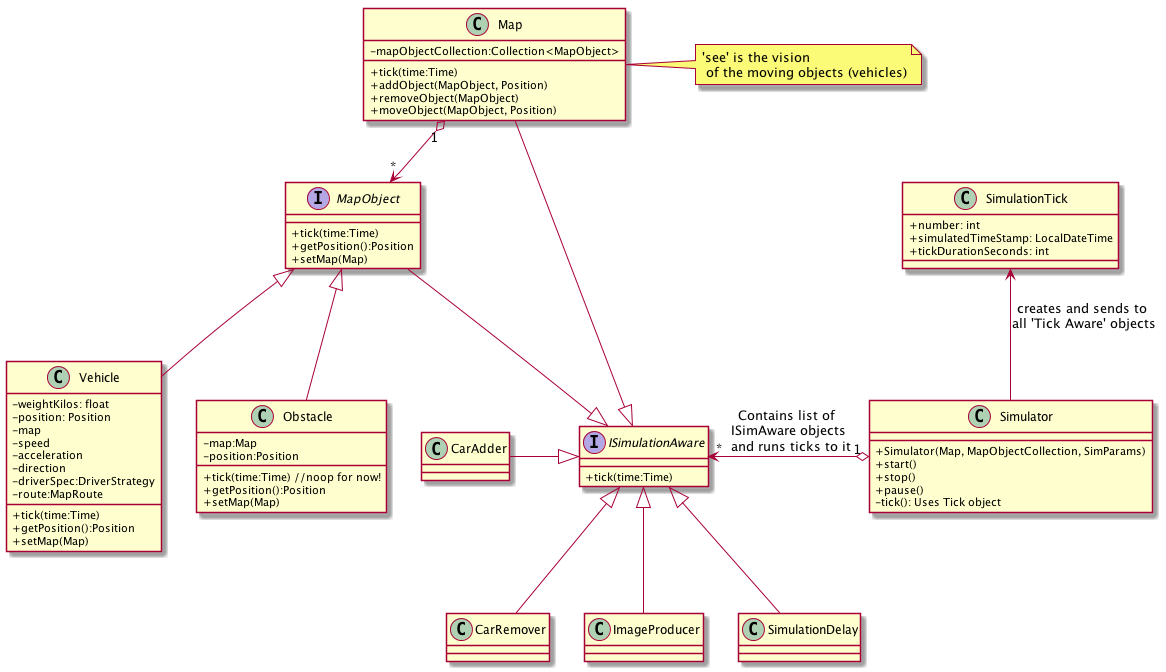
\includegraphics[width=0.75\textwidth]{../../uml_diagrams/simulatorClassDiagram.png}
    \vspace{1.5em}
\end{figure}

Since the Simulator has control over what are the parameters ticks are created with, it is possible to control time granularity or speed. At the same time such approach causes some limitations: as such, if the tick duration is too long, for example, traffic lights might be able to update.
Diagram in Figure \ref{fig:simulationClassDiagram} details main classes forming structure for the actual movement simulation.

\subsubsection{Movement within the single road}
Vehicles are modelled using different physical parameters. At each simulation time moment, vehicle can have certain speed and acceleration values. Using the speed and tick duration, vehicle can determine its next position along the lane, and move there. Using the acceleration, same process is applied to the speed value. Vehicle determines what to do, depending on current road conditions it is in. For example, if it approaches a crossing, it needs to slow down.

There are two types of vehicles introduced to the system: passenger cars and trucks. They share different initialization parameters: trucks are bigger in metric sizes, slower, having way lower maximum acceleration and lower maximum speed than passenger cars.

Vehicles move within and along the lane. Since lane is represented with the polyline, having certain width, vehicle can easily place itself within the one-dimensional coordinate space, the only coordinate being the distance along the polyline from its start. In such a coordinate system, movement looks like a movement along the straight line, and the polyline determines actual change in bearing and meters offset coordinate system.

There might be cases when the vehicle may want to change lane. For example, consider slower truck moving ahead of faster passenger car. As soon as car reaches certain distance to the truck, it might want to change the lane to adjacent one in order to continue moving with higher speed. Vehicles maintain a certain distance to next object which is dependent on speed. All three stages of lane changing are displayed in Figure \ref{fig:carKeepingDistance}. Vehicle color hue depends on the speed, and circle with the bearing vector in it represents the car movement direction and distance to keep to next one.
\begin{figure}[!h]
    \vspace{1.5em}
    \caption{Car changing lane}
    \label{fig:carKeepingDistance}
    \centering
    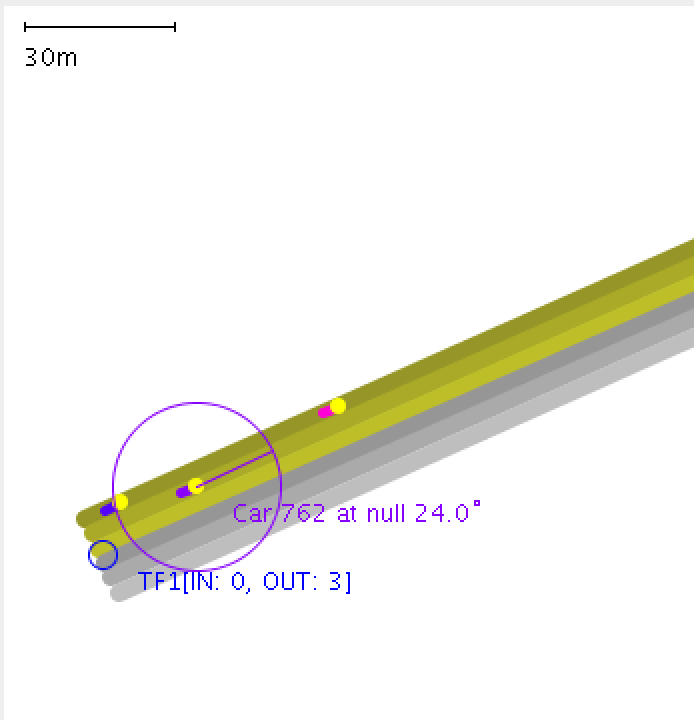
\includegraphics[width=0.3\textwidth]{figs/carMovement/car_keeping_distance_to_other.png}
    \hspace{0.2em}
    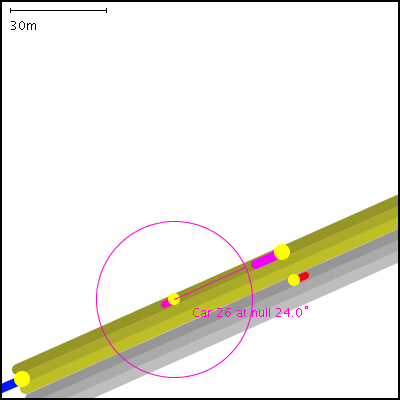
\includegraphics[width=0.3\textwidth]{figs/carMovement/car_lane_change_before.png}
    \hspace{0.2em}
    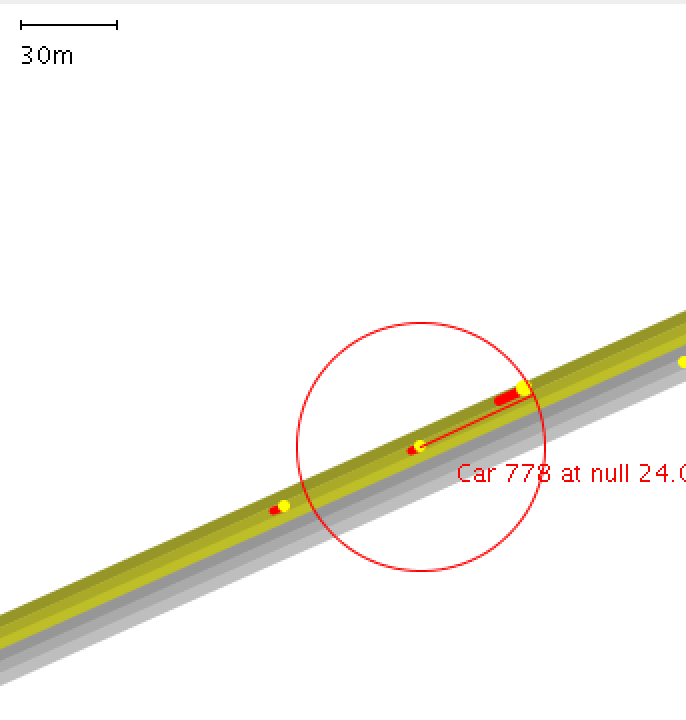
\includegraphics[width=0.3\textwidth]{figs/carMovement/car_lane_change_after.png}
    \vspace{1.5em}
\end{figure}

Definitely, it is not always the case that changing lane is possible. For example, there may be no adjacent lane, or both the adjacent lanes are buys. Following is the process of lane changing represented as decision flow:
\begin{enumerate}
    \item If there is vehicle (any part of it) in current lane within distance to keep,
    \item Check if there is a lane to the inner side of the road. If it exists, and it is free for distance to keep in front and back, change there.
    \item If that did not succeed, apply same procedure for the outer lane.
    \item If that did not succeed, decelerate.
\end{enumerate}

Depending on the data obtained from the OSM file, roads can be one-way roads or bi-directional roads. As a pleasant bonus the software is mostly capable of working with both the right hand side movement and left hand side. The direction of the road is established by sequence of the nodes in polyline. One way roads then become a collection of lanes running in that way. For the two-way roads, the opposite set of lanes is created.

\subsubsection{Movement in junction}
In the current implementation of traffic simulator, junction is purely logical: it is a point where multiple roads having some lanes connect. When a car reaches this point, it can take a decision (within certain limits) what next lane to switch to. All possible paths are pre-computed using the graph tool in the graph construction phase. At the same time, vehicle can, and should have certain specifics and limitations as to what are the possible actions. Consider a kerb to kerb turn radius: a minimal U-turn possible for a Mini Cooper is hard to imagine for 6-axis truck.

When reaching a junction, vehicle needs to decide first what is the plan\footnote{Actual decision process is implemented with weighted random selection, with some preference given to 'move straight' mode. This is the good place to introduce route planning and traffic profiling}. There are two options possible: vehicle wants to carry on in roughly the same direction, or it wants to turn. In real life data, the 'same direction' does not necessarily mean same bearing of the adjacent road segments, sometimes these may be considerably different. In order to attack this problem, an empirical rule was established, which classifies all available junction proceedings whose angle between incoming and outgoing vector is less than 30\degspc  as 'moving straight', and ones with angle between 100\degspc  and 30\degspc as turns. Everything requiring turn with an angle larger than 110\degspc is considered a prohibited turn. As a result, U-turns are not allowed in simulation.

Upon switching to the new lane, car continues to move along it in the same mode as described in previous section.

Figure \ref{fig:forwardOrTurnOption} displays the forward and turn sectors for the car approaching crossing. The crossing itself is displayed as a white circle in the center. Small car is approaching the crossing from the east. The car is following an inbound lane with the bearing at the junction of 15.9\degspc. The junction itself, in addition to two incoming lanes at 15.9\degspc and 158.7\degspc, has two outgoing lanes: one at 19.7\degspc, and one at 107.4\degspc. For the Car 46 approaching the junction, possible forward and turn outcomes are displayed on the overlay disc: red segments represent prohibited proceedings, yellow ones represent turns, and green ones represent forward movement. For this very scenario, Car 46 has an option to go forward with the 19.7\degspc exit, and an option to turn left with 107.4\degspc exit.

\begin{figure}[H]
    \vspace{1.5em}
    \caption{Junction forward or turn options depending on angle }
    \label{fig:forwardOrTurnOption}
    \centering
    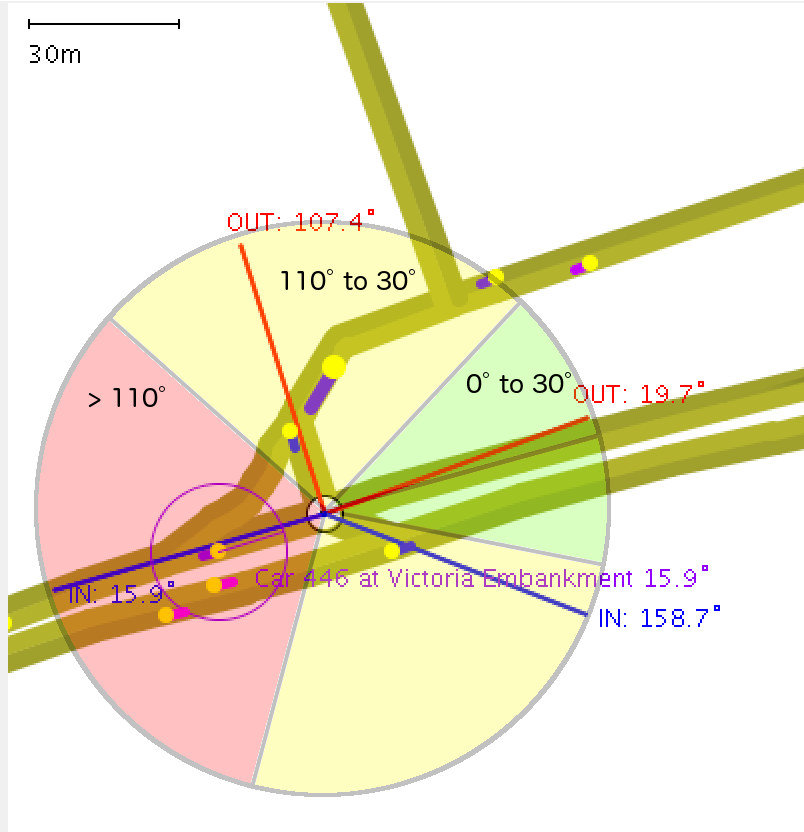
\includegraphics[width=0.4\textwidth]{figs/junction/junction_car_incoming_angle_with_turn_sectors.png}
    \vspace{1.5em}
\end{figure}

In real mapping data junctions can take various forms. Figure \ref{fig:junctionTypes} displays two commonly found types of junctions: a simple connection of two roads, which is quite possible one road split by a traffic light and pedestrian crossing, and more complex junction having 5 streets connected to it. Using the method specified above, car can conveniently move across this junction, either moving forward or attempting a turn in any of the allowed directions.

Within this model, roundabout is established as a set of short one-way connected roads forming a circular structure. Right image in Figure \ref{fig:junctionTypes} shows a typical roundabout, with the road debug display setting enabled, where each individual lane is painted with new color in round-robin manner. One can clearly see where and how the roads connect.

\begin{figure}[h]
    \vspace{1.5em}
    \caption{Junctions found in real mapping data}
    \label{fig:junctionTypes}
    \centering
    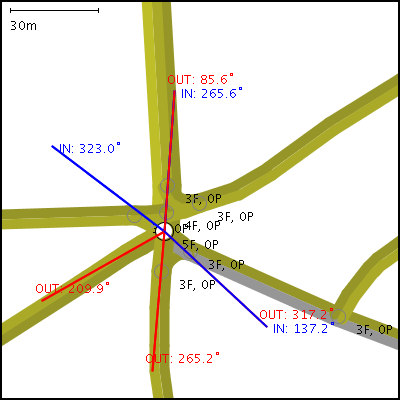
\includegraphics[width=0.3\textwidth]{figs/junction/junction_5_roads.png}
    \hspace{0.2em}
    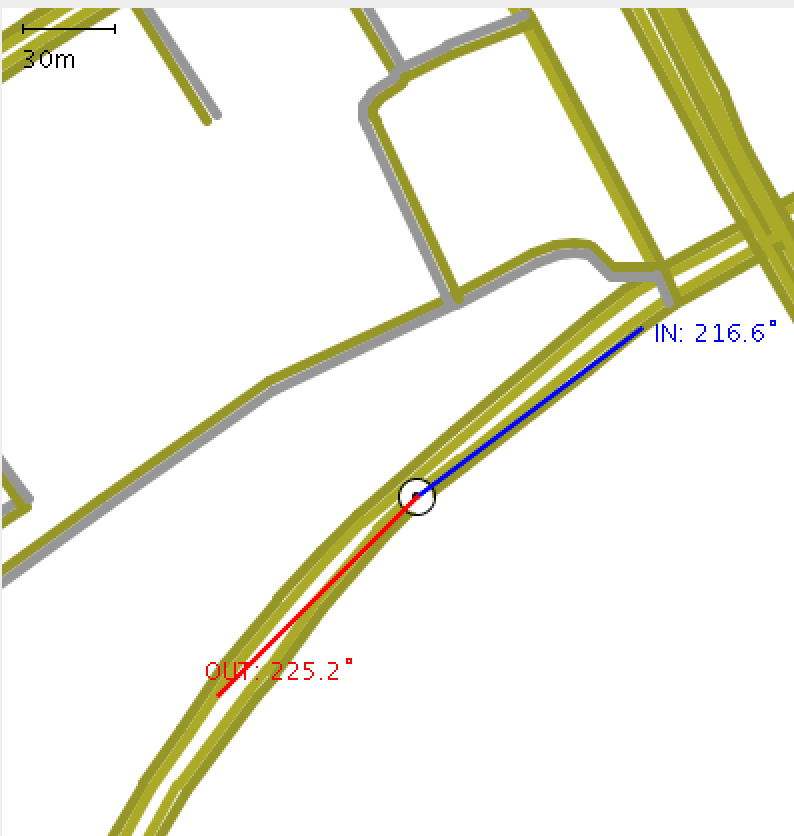
\includegraphics[width=0.3\textwidth]{figs/junction/junction_two_roads.png}
    \hspace{0.2em}
    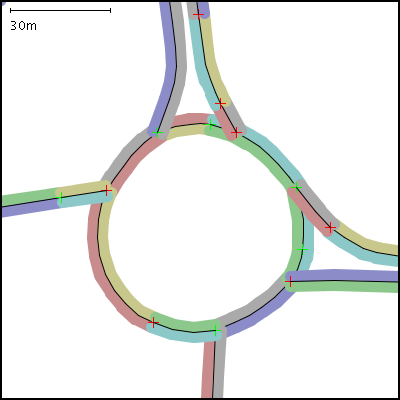
\includegraphics[width=0.3\textwidth]{figs/junction/roundabout.png}
    \vspace{1.5em}
\end{figure}

A more subtle subtype of junctions is a fork, commonly found in proximity to roundabouts. Fork usually consist of multiple inflow or outflow features connected to a junction with a slight difference in degree with single outflow or inflow feature, respectively. Figure \ref{fig:forkTypes}, left, depicts a collecting fork joining two 2-lane one-way roads into the bridge road. The right image displays an actual two-lane two-way road splitting each lane into the two-lane one-way road.

\begin{figure}[h]
    \vspace{1.5em}
    \caption{Forks found in real mapping data}
    \label{fig:forkTypes}
    \centering
    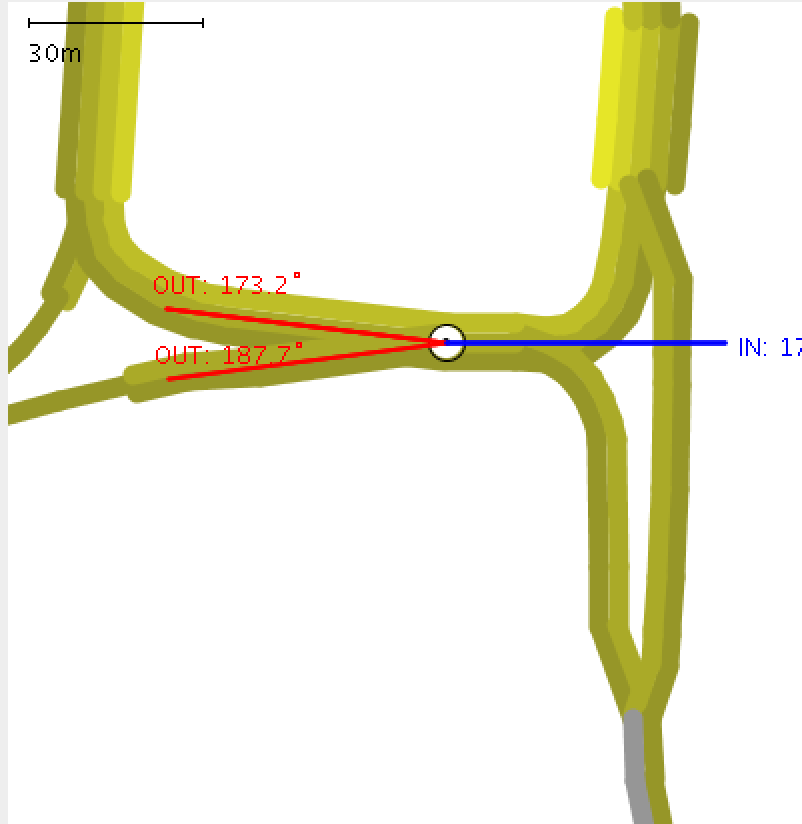
\includegraphics[width=0.4\textwidth]{figs/junction/junction_oneway_to_fork.png}
    \hspace{0.2em}
    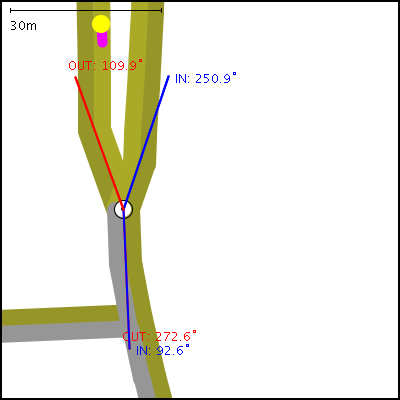
\includegraphics[width=0.4\textwidth]{figs/junction/junction_two_way_to_fork.png}
    \vspace{1.5em}
\end{figure}

\subsection{Logger}

A logger was created at the beginning to help over the life of the development process. As one of the three major resources available for debugging (the others being in-line print and exceptions) it was viewed as an essential to have for the project. A home-brewed logger was chosen over a ready-made one to keep the functionalities to those required and, also, as it was a good addition to the code base.

The logger was used extensively to keep track of what was happening during runtime and have a way to keep a permanent record of states during each run for errors/bugs that were hard to reproduce. Although simple, the architecture was designed to be flexible allowing further developments of outputs and formatters (see Figure~\ref{fig:logger_overview}).

\begin{figure}[!h]
	\vspace{1.5em}
  	\caption{Logger Overview}
  	\label{fig:logger_overview}
  	\centering
	\includegraphics[width=0.75\textwidth]{figs/logger/LogModuleObjectDiagram.png}
  	\vspace{1.5em}
\end{figure}

\subsubsection{Log Messages}
The logger allows for various types (importance levels) of messages which are all defined as calls in the interface:
\begin{itemize}
	\item Fatal messages: for unrecoverable errors (program crashes),
	\item Error messages: for recoverable errors (program can continue somehow),
	\item Normal messages: for standard information messages,
	\item Debug messages: for more specific events that would be more useful for debugging,
	\item Trace messages: to help trace the program flow when bugs arise.
\end{itemize}

Messages to the logger, whether actual messages or exceptions, all carry certain properties to the outputs:
\begin{itemize}
	\item A session message number,
	\item the date/time stamp of the message,
	\item the origin of the message (the class's name usually)
\end{itemize}

\begin{lstlisting}[language=java]
	private static Logger_Interface LOG = Logger.getLoggerInstance(Road.class.getSimpleName());
\end{lstlisting}

An actual message also includes its level with the message description whilst an exception message just carries the stack trace of the exception.

Since, in Java, most types are children of the Object class and 'autoboxing'\cite{Oracle1995} is available for primitive types, <Object> can be used as the type for the signature of the method that are called to pass a message. In logging messages there are no set number of arguments for the description so there are two options opened to us: allow strings only or allow any number of arguments to be passed to the methods for the log calls. The latter was chosen for flexibility's sake in order to be able to pass dynamic variables directly.

\begin{lstlisting}[language=Java]
	LOG.log_Error("Road '", lanes.getRoad().getID(), "' has group of directed lanes with partly implemented Links (Back). ", link_count, "/", lanes.getNumberOfLanes(), " Lanes connected to a link.");
	LOG.log_Trace("X--> '", lanes.getID(), "' has no previous link(s).");
\end{lstlisting} 

In Java the 3 dots (also known as 'vararg' \cite{Oracle2004}) can be used to achieve such goals.

\begin{lstlisting}[language=Java]
	void log_Error(Object... objects);
\end{lstlisting}

\subsubsection{Log Outputs}
There are three outputs with matching formatters available for use:
\begin{enumerate}
	\item Console,
	\item Text file,
	\item Comma separated values (CSV) file.
\end{enumerate}

Any file output due to the nature of writing to disk will incur a more sizeable performance cost than printing to the console. Text is used for general record keeping where CSV aims to help debugging as it is easier to import it into a database or spreadsheet to filter out the messages based on the different properties that are passed along the message description. It also allows for more flexibility if reformatting is required outside the logger.



\subsubsection{Log Configuration}

Configuration injection via a file was implemented so that options could be changed without having to recompile the application. It offers more flexibility as well than hard coded options for the user. Through the configuration file the following options can be manipulated:

\begin{itemize}
   	\item At which log level to record messages,
   	\item Output format (txt, csv, console),
   	\item Output name (file name in the case of txt and csv),
   	\item Whether or not to record Exceptions in the log,
\end{itemize}

In the event that no configuration file is found a default one is created that includes some guidelines on what options are available:

\begin{lstlisting}
	//======================================================================================
	// - Log configuration file - 
	//======================================================================================
	// Output types available: TERMINAL, TXT, CSV
	// Flag types available: EXCEPTIONS,
	// 	> syntax: NAME_OF_FLAG=1 for On or NAME_OF_FLAG=0 for Off
	// Variable types available: LEVEL
	// 	> level types: OFF, FATAL, ERROR, WARNING, MESSAGE, DEBUG, TRACE
	//=======================================EXAMPLES=======================================
	// OUTPUT=<TERMINAL,my_name>
	// VARIABLE<LEVEL,OFF>
	// FLAG=<EXCEPTION,0>
	//======================================================================================
	VARIABLE=<LEVEL,WARNING>
	FLAG=<EXCEPTIONS,1>
	OUTPUT=<TERMINAL,Console>
	OUTPUT=<TXT,log>
\end{lstlisting}


\section{Incomplete Functionalities}

\subsection{Traffic Lights}

We could have improved our program by adding Traffic lights module. The figure below shows the prepared class diagram. All management should have been in traffic light controller class. The rules for changing traffic lights' states were supposed to be in TrafficLightRule and TrafficLightsSetRule classes.

\begin{figure}[!h]
	\vspace{1.5em}
  	\caption{Traffic lights class diagram}
  	\label{fig:tf_diagram}
  	\centering
	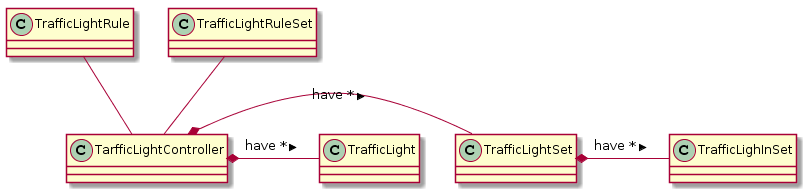
\includegraphics[width=0.75\textwidth]{figs/junction/tf_diagram.png}
  	\vspace{1.5em}
\end{figure}

The idea of Traffic light module contained the following issues:
\begin{itemize}
    \item Two types of traffic lights: singles and those in one junction set.
    \item All traffic lights work autonomously.
    \item Traffic lights in one junction set would have the same ID as Junction.
    \item The first idea was to create basic traffic lights rules, that do not change states according to the traffic (not intelligent traffic lights)
\end{itemize}

\subsection{Serialization}
During the development and testing it was understood that program compilation/running takes a lot of time and affects the performance. Therefore, an idea to save the current state of a map and load it later using GUI was introduced during the team meetings. Initial steps were done, but as project became more complex this feature was left undeveloped.

\subsection{GUI Primitives}
Initially when we went for a micro  model we dealt with each car individually. Thus to reduce the overhead at the simulator, we planed to make a class with various functions that could be called to make the cars, and the roads, based on the location and other details of the same. This function was initially thought for drawing roads, cars, and trucks. It has an initial problem due to miscommunication, which led to a wrong design start. Upon rectifying out mistakes, we were again met with another problem of design, and implementation. The basic formula of the design was based around the coordinates of the placement of the car, thus it lead to cars being produced of different sizes based on the location on the map. Thus to remove the drawing issue it was decided to go with a picture of the car rather than a drawing, as it was an easier option. The image made a few things easier such as placement and sizing, but added new problems like initial direction of the image, and its background transparency. We had already spent a lot of time in this, and it was not getting to some concrete work. Even then we didn't loose hope and tried to get it working. As time progressed there were other problems with the code that had to be dealt with. The initial coding was very basic, and had to be streamlined and improved upon. This was added to the already existing list of problems to be dealt with. Once the code was streamlined, the next step initially was to make it log all the failures that occurred while running. Upon this, just to check the performance of the code we ran a small test. The results were not what one would expect. The execution time for each iteration was very high. At this moment of time, the most important thing to be done was to reduce the execution time, because with such long execution time the code couldn't be considered. It took us long to improve the execution time, and till then it was too late. While applying this whole concept we lost our way, and recovery was slow, may it be the initial misunderstanding or the latter neglect of the image while trying to reformat the code.

\section{Team Work}
%Describe how you worked together, including the tools and processes you used to facilitate group work.

\subsection{Tools and processes}

The team unanimously used IntelliJ IDEA\footnote{https://www.jetbrains.com/idea/} for coding and version control access. The IDE offers a wide array of development tools that automate a lot of "boiler-plate" things for Java enabling the user to focus on the more important aspects of development. It also has an integrated VCS module.

The team originally adopted a simplified Kanban\cite{Peterson2015, Radig2016} process towards Agile development where tasks are broken down and piled into a backlog where any member(s) of the team can take them on and move them to the "In progress" pile. Once tasks are done they can be moved to the "code-review" pile and finally to the "Done" pile.

To aid in that process, Trello\footnote{https://trello.com} was used to keep track of the tasks (see Figure~\ref{fig:trello}). As time went on updates on the board became more sporadic and its usage amongst the team was not equally spread so it ended up not being used to its fullest potential. 

For day-to-day communication HipChat was used as the team's IM. It has both Trello and GitHub\footnote{https://github.com} integration so that any updates in either were automatically posted inside of it. This enabled the members to, at a glance, see any of the activities that occurred. It was used to "shout out" to team members when any had urgent questions or thoughts to share during development.

\begin{figure}[!h]
	\vspace{1.5em}
  	\caption{Snapshot of the Trello board during development}
  	\label{fig:trello}
  	\centering
	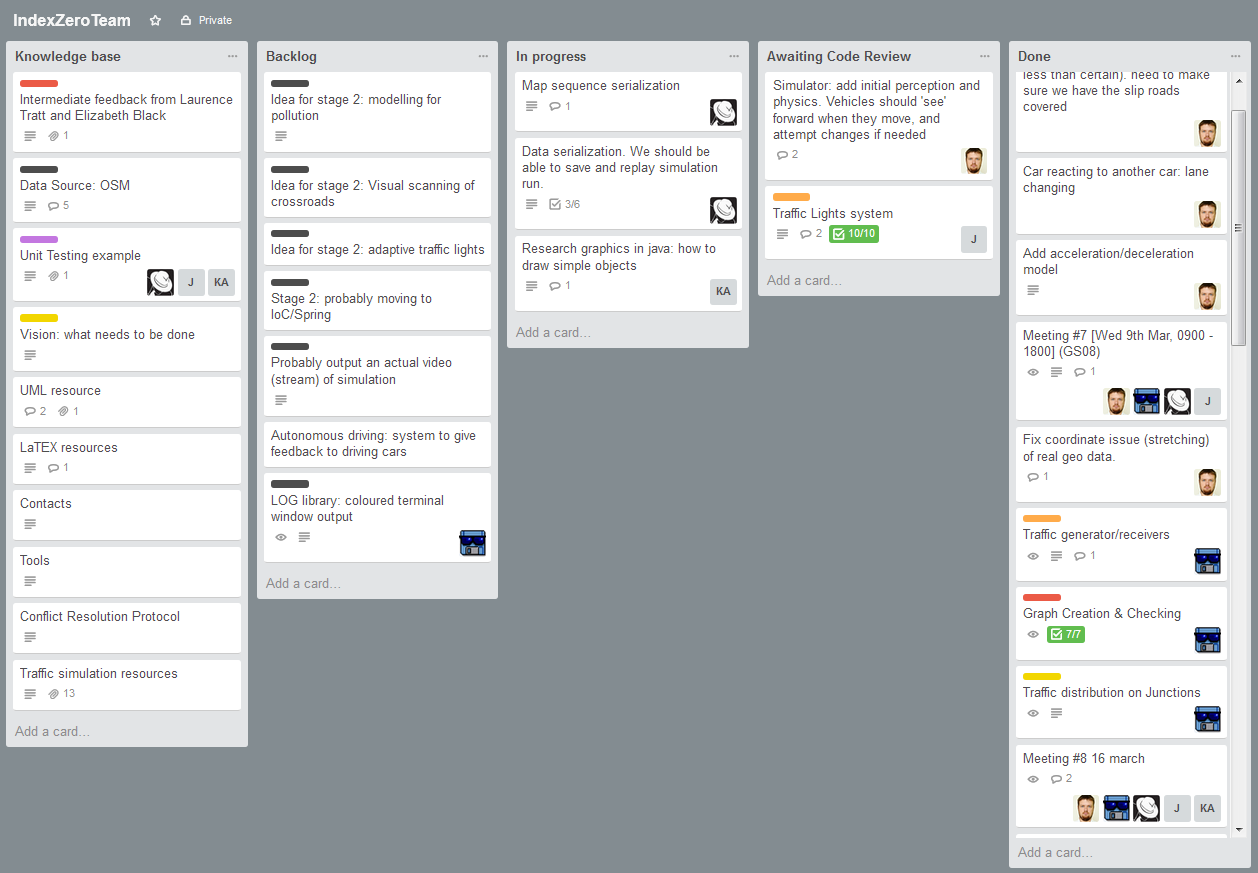
\includegraphics[width=1\textwidth]{figs/Tools/trello.png}
  	\vspace{1.5em}
\end{figure}

\subsection{Learning Outcomes}

Aside from the system-specific knowledge gained and previously outlined by creating a working traffic simulation application, the team's learning outcomes come in two major categories: technical and non-technical (soft skills).

For the technical aspects:
\begin{itemize}
	\item Build systems (Gradle),
	\item Git - especially working with feature branches and pull request (Github),
	\item Java 8 - new functionalities available such as lambdas, method references and streams,
	\item Unit testing methodologies - plain unit testing and with mock objects
	\item LaTeX for typesetting
\end{itemize}

On the non-technical side:
\begin{itemize}
	\item Kanban approach to agile development,
	\item Collaborative software development,
	\item Knowledge sharing in a team,
	\item Organisation (room booking, making sure everyone know what they are doing, etc...),
	\item Problems that occur within teams (as outlined in the next section).
\end{itemize}

\subsection{Team Performance Evaluation}

The team originally set out for equal input in the project where both technical and non-technical tasks were viewed on the same scale. This would have allowed less technically experienced members to contribute on the same level as more experienced members. A plan was devised and parts for the project were broken down into specific tasks to be taken up based on expertise. If no one had the expertise it came down to whomever wasn't on a task at that particular time.

Some of the aspects that worked well included:
\begin{itemize}
	\item Regular group meeting every week (sometimes twice) in the library's group study rooms.
	\item Ever increasing time booked for coding in group was pushed,
	\item The majority of the time, all members were present in the meetings,
	\item When technical problems arose for members questions were raised and dealt promptly and
	\item Help was offered freely by more technically knowledgeable peers.
\end{itemize}

Unfortunately this methodology lost track over the course of the project's lifetime. Some of the problems identified were:
\begin{itemize}
    \item Tendency towards procrastination and a lack of pro-activity in picking up tasks without prompting became evident,
    \item Extended periods of low output for the project led to loosing track of the changes and difficulty understanding current states of the project on a model level for some of the members,
    \item Other peripheral tasks (both technical and not - e.g. research, docs, report.. ) tended to be ignored or relegated to the low priority list in cases by part of the team with the assumption that it would get done by someone else,
    \item Code review was not as effective as it could have been in fostering legacy learning from more experienced members due to the sporadic contribution in cases,
    \item Tasks on the agenda where not always done prior to the meetings which delayed those in the pending stack even further,
    \item Once the discussion section of the meeting sessions were finished, the rest of the time reserved which was meant for group coding was not used to its best.
    \item Although motivation to achieve and get work done for the project was at a high point at the end of meetings it didn't sustain for some members.
\end{itemize}

In the end, the combination of these issues lead to an asymmetric distribution of work input on the project.

Following are some numerical properties about project implementation course:
\begin{itemize}
    \item 110 Java source files created
    \item 11111 lines of Java code written
    \item 420+ commits
    \item 13 pull requests
    \item 50+ cards created in Trello
    \item 108 unit tests
    \item Test suite coverage:
    \begin{itemize}
        \item Simulator: 66\% statement coverage, 49\% branch coverage
        \item Logger: 50\% statement coverage, 58\% branch coverage
        \item Gui: 0\% statement coverage, 0\% branch coverage
    \end{itemize}
\end{itemize}

\section{Project Evaluation}
\label{sec:projectEvaluation}
%Critically evaluate your project: what worked well, and what didn’t? How did you do relative to your plan? what changes were the result of improved thinking and what changes were forced upon you? how did your team work together? etc. Note that you need to show that you understand the weaknesses in your work as well as its strengths. You may wish to identify relevant future work that could be done on your project.

Originally the project was to take up the cellular automata model for the simulation. As it became obvious this would cause a problem for vehicles especially at stop point where it would leave gaps between the objects due to the nature of static sized cells the project evolved towards a more precise model with coordinates for movement placement allowing for a more granular and realistic simulation.

The code, whilst based on a simple set of designs, was a driving force towards changes as flaws in the original ideas and design were discovered as development went. One example of this is the change from linking roads bidirectionally as whole features to creating lanes and moving the graph linkage to those in a directed fashion.

Because of these changes whole sections of the code-base would become either redundant and deleted or modified to such extent that the original clean implementation had morphed into something less so. Given time those would need some refactoring to avoid the possibility of code-rot if this software was going to be further developed.

One particular point of interest would be the movement along the lanes. Currently, as the offset construction of the individual lanes within a road is made based on the polyline, a vehicle when travelling on the backward lane requires a calculation that subtracts from the total length whereas, on the forward direction, the calculation adds from 0. The latter being more natural.

Certain planned functionalities were not achieved in the end as the work input capacity was not as originally anticipated and the creation of the graph from OSM data was more involved than previously thought. In the end most of the basic and advanced items planned were completed in addition to some extra ones (see Table~\ref{table:functionalities}).

\begin{table}[!h]
\vspace{1.5em}
\centering
\caption{Functionalities implemented before/after comparison}
\label{table:functionalities}
\resizebox{0.75\linewidth}{!}{%
\begin{tabular}{|l|c|c|c|}
\rowcolor[HTML]{656565}
\hline
{\color[HTML]{FFFFFF} \textbf{Functionalities}} & {\color[HTML]{FFFFFF} \textbf{Original}} & {\color[HTML]{FFFFFF} \textbf{Final}} & {\color[HTML]{FFFFFF} \textbf{Done}} \\ \hline
\multicolumn{4}{l}{\textbf{Basic functionalities}}                                        \\ \hline
Gradle deployment harness                       & \checkmark  & \checkmark  & \checkmark  \\ \hline
Logger: basic functionality                     & \checkmark  & \checkmark  & \checkmark  \\ \hline
Logger: Multi-output support                    & \checkmark  & \checkmark  & \checkmark  \\ \hline
Tooling                                         & \checkmark  & \checkmark  & \checkmark  \\ \hline
Simulation                                      & \checkmark  & \checkmark  & \checkmark  \\ \hline
Basic GUI                                       & \checkmark  & \checkmark  & \checkmark  \\ \hline
Basic measurement (throughput)                  & \checkmark  & \checkmark  & \checkmark  \\ \hline
Simulation saving/loading                       & \checkmark  &             &             \\ \hline
\multicolumn{4}{l}{\textbf{Advanced functionalities}}                                     \\ \hline
Larger model: Graph with many connections       & \checkmark  & \checkmark  & \checkmark  \\ \hline
Loading map data from OSM                       & \checkmark  & \checkmark  & \checkmark  \\ \hline
Traffic Lights and model parameter optimisation & \checkmark  &             &             \\ \hline
Advanced GUI (inspection, graph debug...)       &             & \checkmark  & \checkmark  \\ \hline
Traffic behaviour: Lane changes                 &             & \checkmark  & \checkmark  \\ \hline
\end{tabular}}
\vspace{1.5em}
\end{table}

\subsection{Application Performance}
After the implementation of the traffic simulator, performance measurements were taken. The parts of the functionality carrying most of the computational load were wrapped in time marker code and their execution time was measured. Single sample was taken each time, since performing subsequent measurements yielded exactly the same results. Following are some details on the time measurement procedure undertaken:

\begin{itemize}
    \item Time recording. In order to circumvent the possible observer bias, the simplest possible measurement method was chosen. The code was augmented to record the timestamp with System.currentTimeMillis() before running the method of interest, and take the sample after it. The difference was computed, and echoed to the standard output with System.out.println().
    \item Logging was disabled at all during performance measurement (level set to OFF).
    \item Test machine: OS X, Intel Core I7-4770HQ, 2.2 GHz, 16GB RAM, SSD
    \item As measurements have shown, the software is capable to deliver a usable experience for a decent sized data set (in our example all primary, secondary and tertiary roads in Greater London, totalling 31101 road and 24314 junction descriptions), as described in Table \ref{table:performanceComparison}
\end{itemize}

\begin{center}
\begin{longtabu} to \textwidth {|
    X[2,l]|
    X[4,l]|
    X[3,c]|
    X[3,c]|
    X[3,c]|
    }
    \hline
    \textbf{Sample} & \textbf{Size} & \textbf{XML load} & \textbf{Graph linkage} & \textbf{Roads draw time} \\ \hline
Straight road & 1 road and 0 junction, 9 mapFeatures, 12 mapLinks, 2 traffic generators & 4 & 0 & 2 \\ \hline
Elephant and Castle & 101 road and 80 junction, 454 mapFeatures, 18 mapLinks, 12 traffic generators & 37 & 4 & 8 \\ \hline
Paris, Arc & 284 road and 168 junction, 1145 mapFeatures, 57 mapLinks, 35 traffic generators & 118 & 68 & 70 \\ \hline
Manhattan, Battery Park & 212 road and 148 junction, 829 mapFeatures, 81 mapLinks, 40 traffic generators & 11 & 5 & 29 \\ \hline
Strand area & 781 road and 530 junction, 2998 mapFeatures, 196 mapLinks, 105 traffic generators & 62 & 19 & 41 \\ \hline
Buckingham Palace& 275 road and 176 junction, 1032 mapFeatures, 68 mapLinks, 41 traffic generators & 28 & 8 & 21 \\ \hline
Whole Manhattan & 14763 road and 10429 junction, 58394 mapFeatures, 1055 mapLinks, 596 traffic generators & 13607 & 468 & 531 \\ \hline
Whole Greater London & 31101 road and 24314 junction, 120672 mapFeatures, 547 mapLinks, 391 traffic generators & 32911 & 644 & 1087 \\ \hline

\caption{Performance metrics of the loading and rendering methods for different map samples}
\label{table:performanceComparison}
\end{longtabu}
\end{center}


\subsection{Possible Further Development and Improvements}

As the core design of the project offers a strong basis for further development there are many avenues of improvement opened that could be taken up.

Firstly the GUI could be improved:

\begin{itemize}
	\item As the program skirts into a hybrid model, the visual detailing, i.e. car sprites, road graphics may be dynamically removed or added. For instance: when the zoom factor increases beyond a threshold the dots representing the vehicles are changed to actual sprites matching their descriptions.
	\item Map editorial functinoality may be added, e.g. a point/click interface for adding static map objects to the graph via the GUI such as road block, construction work or broken down cars.
	\item The GUI map editor could enable easy OSM error corrections or even synthetic map creation.
\end{itemize}

The second group of possible improvements are those related to the simulator:

\begin{itemize}
	\item Complex traffic lights with not only green and red but also early/late yellow states could have been added to the program. This could have been further expanded to intelligent traffic lights devising on their mode basing on throughput data.
	\item There is a maximum number of cars that are allowed on map (currently 500), but in general that could have been improved by creating a vehicle generator that depends on the map size.
	\item There is also a possibility of vehicles specification based on real-life data.
	\item APIs could have been provided to enable plug-in behaviours for vehicle driving strategy and metrics. Components in that case would be added easily.
	\item Pollution profiler with a visualized heat map would be a nice addition.
    \item The maps could be read from other sources, for example Google or Bing maps.
    \item Using intermediate format for simuilation state persistence would allow to record and later re-play the simulation sessions, enabling communication.
	\item Logger coloured terminal output accessible from the GUI.
	\item Custom log message filters (based on origin, granular individual log level control)
\end{itemize}

\section{Peer Assessment}
%In a simple table, allocate the 100 ‘points’ you are given to each team member. Valid values range from 0 to 100 inclusive. You may assign decimal values, but the entire points must add up to precisely 100.
Table \ref{table:peerAssesment} is the Peer Assessment table as required by the project description.

\begin{table}[hb]
\centering
\caption{Peer assessment}
\label{table:peerAssesment}
\begin{tabular}{lc}
\hline
Esmond Davison & 32\\
Farhad Rahimli & 12\\
Kumar Awijeet &  12\\
Jacek Krupski &  12\\
Oleksandr Cherednychenko &  32\\
\hline
\end{tabular}
\end{table}

% Apply paragraph spacing only for the main report body %
\setlength{\parskip}{0em}
